\chapter[Transponder VDL 4000/VTE CNS SYSTEMS]{Transponder VDL 4000/VTE CNS SYSTEMS}

\begin{itemize}

\item \textbf{Tipos de Transponder}

Existem transponders passivos e ativos:

\textbf{Passivos:} Transponders passivos são frequentemente encontrados, sendo equipamentos relativamente simples, podendo ser observados na forma de etiquetas ou chips, desprovidos de baterias ou fontes próprias de energia, são energizados e ativados quando na presença do leitor, por meio da emissão de radiofrequência. Frequentemente utilizados no meio comercial/industrial, bem como em chaves codificadas.

\textbf{Ativos:} Transponders ativos são em geral mais complexos que os modelos passivos, pois envolvem a emissão de dados via radiofrequência tanto na requisição de dados bem como no envio da resposta. Com aplicação difundida nos campos aeronáutico e naval, servem como base de comunicações/identificação a longa distância. Por serem equipamentos ativos, necessitam de uma fonte energética constante. Possuem uma taxa de transmissão de dados muito superior aos modelos passivos.

Para aplicação em nosso caso, abordaremos apenas o conceito de transponders ativos.

\item \textbf{Funcionamento}

Um transponder ativo funciona à base de emissão de radiofrequência, tanto para solicitar os dados de outros dispositivos bem como para emitir os dados armazenados em si. Desta forma, é necessário notar que um transponder não fornece dados, sejam eles quaisquer sejam, mas se apresenta como uma solução versátil para comunicação à longa distância, transmitindo dados armazenados/coletados pelo sistema ao qual está acoplado.

No caso da aplicação aeronáutica, os transponders são utilizados para transmitir às estações de controle em solo dados como posição, altitude, velocidade e direção das aeronaves, sendo que esses dados são obtidos por diferentes sensores.
	
\item \textbf{Aplicação no caso}

Os dados coletados pelo velocímetro e GPS, necessários aos cálculos base do sistema, serão transmitidos à distância necessária e com alto grau de confiabilidade, uma vez que, ao utilizar radiação eletromagnética para transmitir os dados, um transponder não sofre com interferências climáticas, ambientais e demais, o que o torna uma boa opção para integrar um sistema crítico.

\item \textbf{Modelo escolhido}

As especificações técnicas do modelo escolhido podem ser encontradas na figura abaixo.

\begin{figure}[h]
  \centering
  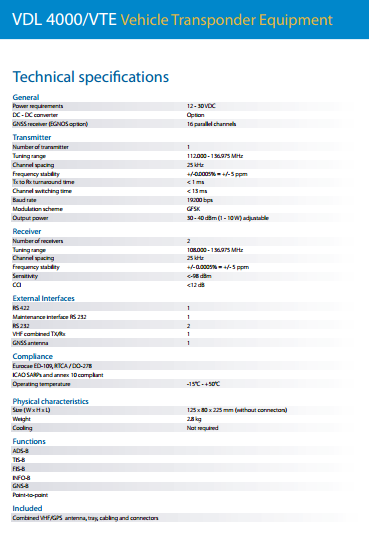
\includegraphics[width=350px, scale=1]{figuras/transponder_settings}
  \caption{Especificações do Transponder}
\label{fig:transponder_settings}
\end{figure}

\end{itemize}